% !TEX root = ../thesis_main.tex
%
%
%
%%%% --- * --- %%%%	
\clearpage
\chapter{Atomic Physics Overview}
\label{atomicphysics_chapter}
\section{Magneto-Optical Traps}
Since its initial description by Raab et. al. in 1987~\cite{raabprentiss}, the magneto-optical trap (MOT) has become a widely used technique in many atomic physics laboratories.  The MOT produces confined samples of cold, electrically neutral and isotopically pure atoms confined within a small spatial region.  It is these properties that make the MOT a valuable tool not only in atomic physics, but for precision measurements in nuclear physics as well, and the TRINAT lab \aside[color=org]{Have I defined TRINAT yet?} has adopted the technique wholeheartedly.

A typical MOT can be created from relatively simple components:  a quadrupole-shaped magnetic field generated at will by two current-carrying coils of wire, and a circularly polarized laser tuned to match one or more atomic transitions in the isotope of interest.  Because a MOT is easily disrupted by interactions with untrapped atoms, the trap must be created within a vaccuum system.  Finally, a source of atoms to be trapped is required.  

\note{... used predominantly with alkalis due to their simple orbital electron structure.}

\note{``In order to understand the mechanism by which a MOT is able to confine atoms, we must first introduce the Zeeman effect (Section 2.1) and a descrip- tion of an optical molasses (Section 2.2). A functional MOT combines the forces resulting from these two mechanisms to trap and cool atoms.''}

%The TRINAT lab has adopted this technique from atomic physics to perform nuclear physics experiments.  
%Such samples may subsequently be used in a variety of physical measurements.
%\note{``Since the magneto-optical trap (MOT) was first described in 1987 by Raab et. al.~\cite{raabprentiss}, it has become a standard technique for confining cold samples of neutral atoms.  These cold trapped atoms may subsequently be used in the measurement of a variety of physical quantities."}

	\subsection{Doppler Cooling}
	\subsection{Zeeman Splitting}
	Needs a level diagram.
	\subsection{Atom Trapping with a MOT}
	\subsection{The AC-MOT}
	Citation for Harvey and Murray goes here~\cite{harveymurray}.  Also, myself~\cite{thesis}.

\section{Optical Pumping}
\note{Needs a better level diagram.}
\begin{figure}[h!!t]
	\centering
	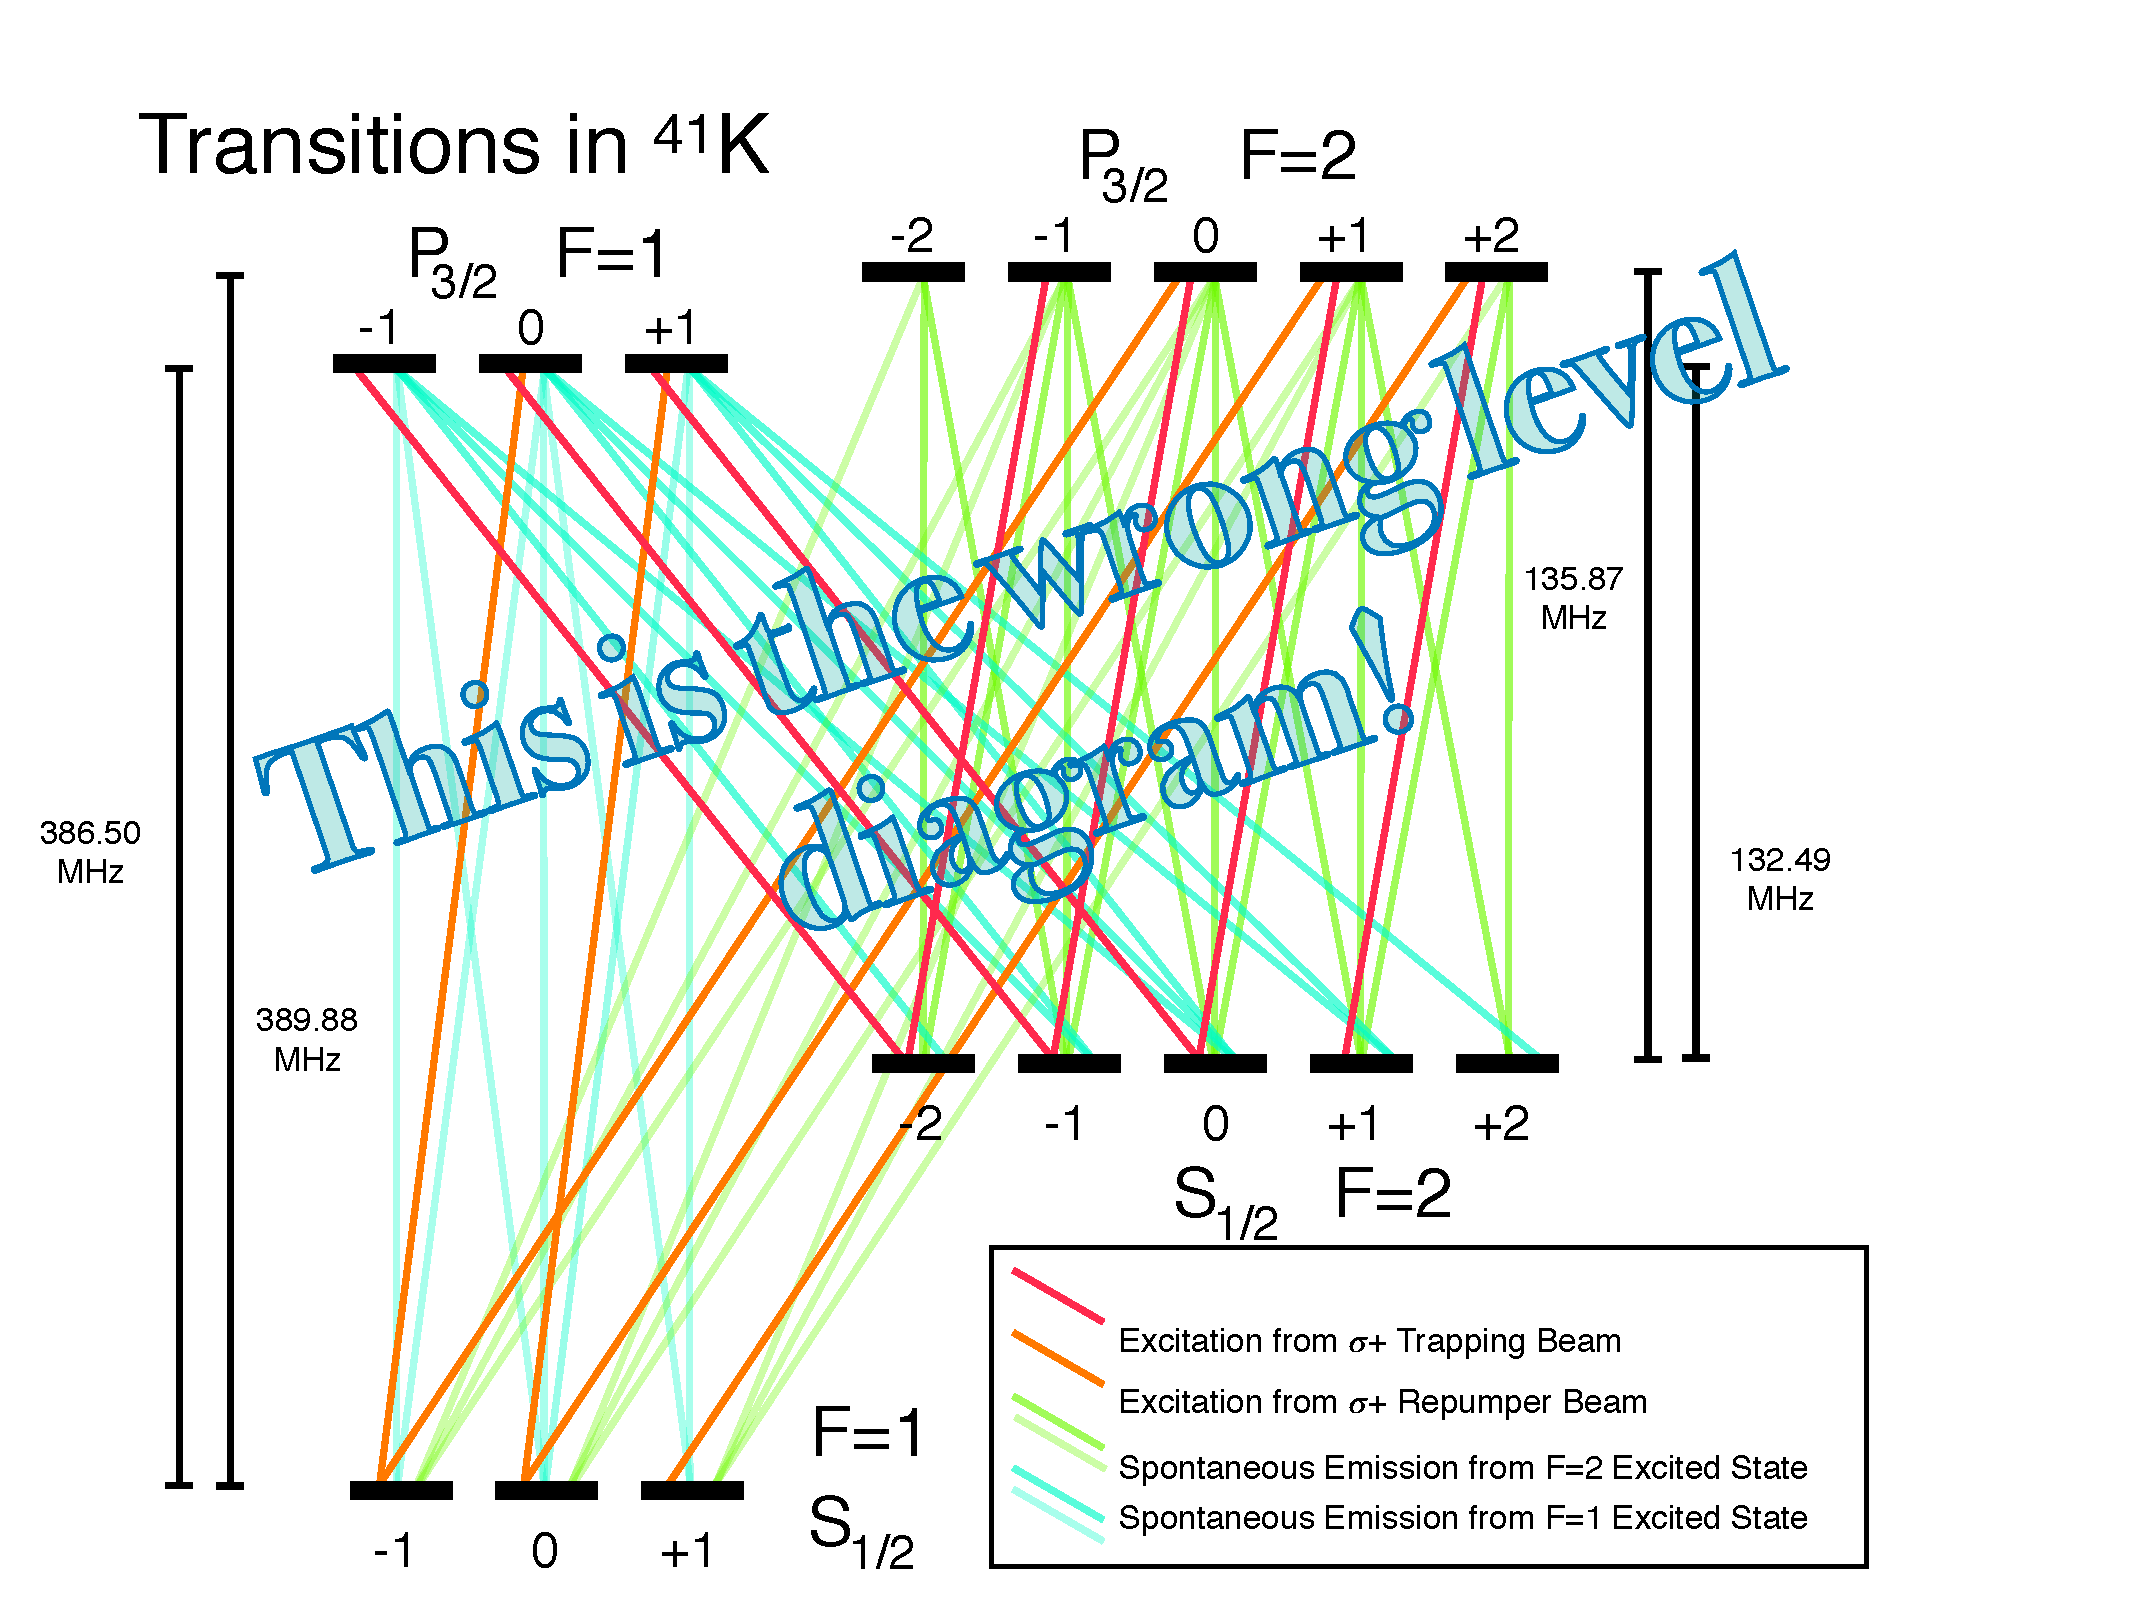
\includegraphics[width=.999\linewidth]
	{Figures/OP_LevelDiagram}
	\caption{An atomic level diagram for the optical pumping of $\isotope[37]{K}$.  Also, this is a diagram for both the wrong isotope, and *probably* also the wrong transition.}	
	\label{fig:op_leveldiagram}
\end{figure}


\section{Shake-off Electron Spectrum}
Shake-off electrons:  where do they come from, and where do they go?  ~\cite{Levinger}.

John made some nice plots of these from the eMCP data.  I did *not* use it to make a cut on eMCP hit position in the end, despite the fact that it makes the spectrum more clean, because a lot of good events don't have full hit position information, and you lose an awful lot of statistics by making the cut.  I used this for modeling the background spectrum, but in the end it wasn't as elegant a result as I might have hoped.  Also, it's still an open question exactly which fraction of SOEs come from which atomic shell, but it doesn't change the resulting spectrum very much.
\missingfigure{SOE Spectrum goes here.}

\note{``Until recently, one limitation of such samples was the necessity for the presence of a relatively large magnetic field, which is expected to partially destroy atomic polarization, limiting the precision of many types of measurements.  Here we discuss the construction of a newer type of MOT, the AC-MOT, which minimizes residual magnetic fields.  The guys in~\cite{harveymurray} came up with the idea of the AC-MOT.  They made it work and did some stuff with it.  Good for them.''}